\documentclass{beamer}
%
% Choose how your presentation looks.
%
% For more themes, color themes and font themes, see:
% http://deic.uab.es/~iblanes/beamer_gallery/index_by_theme.html
%
\mode<presentation>
{
  \usetheme{Boadilla}      % or try Darmstadt, Madrid, Warsaw, ...
  \usecolortheme{beaver} % or try albatross, beaver, crane, ...
  \usefonttheme{default}  % or try serif, structurebold, ...
  \setbeamertemplate{navigation symbols}{}
  \setbeamertemplate{caption}[numbered]
  
} 

\usepackage{xcolor,colortbl}
\usepackage[english]{babel}
\usepackage[utf8x]{inputenc}
\usepackage{courier}
\usepackage{dsfont}
\usepackage{verbatim} 
\usepackage{enumerate}
\usepackage{tikz}
\usetikzlibrary{shapes.geometric, arrows}
\usepackage{multirow}
\usepackage{venndiagram}
\usepackage{epigraph} 
%\usepackage{xcolor}
\usepackage{makecell}

%\usepackage{enumitem}

\usepackage{hyperref}
\hypersetup{
    colorlinks=true,
    linkcolor=blue,
    filecolor=magenta,      
    urlcolor=cyan,
}

% R stuff!
\usepackage{listings}
\definecolor{codegreen}{rgb}{0,0.6,0}
\definecolor{codegray}{rgb}{0.5,0.5,0.5}
\definecolor{codepurple}{rgb}{0.58,0,0.82}
\definecolor{backcolour}{rgb}{0.95,0.95,0.92}

\lstdefinestyle{mystyle}{
    backgroundcolor=\color{backcolour},    
    commentstyle=\color{codegreen},
    keywordstyle=\color{black},
    numberstyle=\tiny\color{codegray},
    stringstyle=\color{codepurple},
    basicstyle=\ttfamily\footnotesize,
    breakatwhitespace=false,         
    breaklines=true,                 
    captionpos=b,                    
    keepspaces=true,                 
    numbers=left,                    
    numbersep=5pt,                  
    showspaces=false,                
    showstringspaces=false,
    showtabs=false,                  
    tabsize=2
}

\lstset{style=mystyle}


\setbeamertemplate{enumerate items}[default]
\setbeamertemplate{itemize item}[triangle]


\title[Introduction to Statistics]{Hypothesis Testing pt. 5}
\subtitle{Decision Making}
\author{Grinnell College}
\date{}

\graphicspath{{img/}}

\begin{document}

\begin{frame}
  \titlepage
\end{frame}

\begin{frame}{Strength of Evidence Approach to Testing}
Up until this point hypothesis testing has followed this basic process:

\begin{enumerate}
\item Begin with a null hypothesis, $H_0: \mu = \mu_0$
\item Collected data and compute a statistic, i.e, $\overline{x}$
\item Compare our statistic against the null distribution, i.e., $T = \frac{\overline{x} - \mu_0}{\hat{\sigma}/\sqrt{n}}$
\item Derive a $p$-value based on the statistic and the distribution
\item Write a summary talking about 'strength of evidence'
\end{enumerate} \vspace{8mm}

We are going to look at an alternative approach where we change Step 5.
\end{frame}

\begin{frame}{Decision Making}
For the remainder of these slides we will talk about this alternative method but I want to point out the following things.
\begin{itemize}
    \item Many statisticians over the past few years have embraced the 'strength of evidence' approach
    \item There are many problems that come with the following approach
    \item However, it is still a relatively common thing you will encounter outside of this class
    \item I will test you on both methods, and will make clear which one I want you to use for a given problem
\end{itemize}
\end{frame}

\begin{frame}{Decision Making -- Motivation}
Based on the evidence we have collected, we must ultimately decide between one of two decisions:
\vspace{2mm}
\begin{enumerate}
\item There is sufficient evidence to reject $H_0$ in favor of $H_A$
\begin{itemize}
    \item data seems unlikely if $H_0$ is true
\end{itemize} \vspace{2mm}
\item There is \textit{not} sufficient evidence to reject $H_0$
\begin{itemize}
    \item data largely agrees with $H_0$
\end{itemize}
\end{enumerate}
\end{frame}

\begin{frame}{Decision Making}
Just as our confidence intervals were correct or incorrect, so to may be our decision regarding $H_0$. In this case, however, there are two distinct ways in which our decision can be incorrect:

\vspace{2mm}

\begin{enumerate}
\item $H_0$ is \textit{TRUE} (i.e., there is no effect), yet we reject anyway \vspace{3mm}
\item $H_0$ is \textit{FALSE} (i.e., there is an effect), yet we fail to reject it
\end{enumerate} 

\end{frame}


\begin{frame}{Decision Making}

These two types of errors are known as Type I and Type II errors, respectively: \vspace{4mm}

\begin{enumerate}
\item $H_0$ is \textit{TRUE} (i.e., there is no effect), yet we reject anyway
	\begin{itemize}
	\item Type I error
	\item ``False positive"
	\item Evidence leads to wrong conclusion
	\end{itemize} \vspace{4mm}
\item $H_0$ is \textit{FALSE} (i.e., there is an effect), yet we fail to reject it
	\begin{itemize}
	\item Type II error
	\item ``False negative"
	\item Not enough evidence to conclude
	\end{itemize}
\end{enumerate} 

\end{frame}

\begin{frame}{Decision Making}

\begin{center}
\def\arraystretch{1.25}
\begin{tabular}{|l|c|c|}
	\hline
	& \multicolumn{2}{c|}{True State of Nature} \\ 
    \cline{2-3} 
    Test Result  & $H_0$ True  & $H_0$ False \\ 
    \hline
    Fail to reject $H_0$ & Correct & Type II Error \\ \hline
    Reject $H_0$ & Type I Error & Correct \\ \hline

\end{tabular}
\end{center}

\end{frame}



\begin{frame}{Type I Errors}

A Type I error describes a situation in which we incorrectly identify an effect:
\begin{itemize}
\item Conclude that an intervention (treatment) works when it does not
\item Conclude that there is a relationship between two variables when there is not
\end{itemize}

\vspace{4mm}

A Type I error will occur, for example, when our constructed confidence does not contain $\mu_0$ when $\mu_0 = \mu$ (true mean equals hypothesized mean)

\end{frame}

\begin{frame}{Type I Errors}
\begin{center}
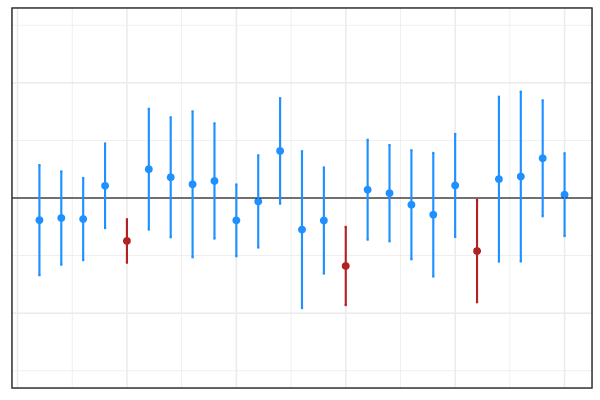
\includegraphics[scale=0.5]{tie.png}
\end{center}
\end{frame}

\begin{frame}{Type I Error Rate}
We can control the rate at which we commit Type I errors with adjusting the \textit{level of significance}, denoted $\alpha$. \vspace{6mm}

This is also called the \textit{Type I error rate} \vspace{6mm}

The Type I error rate has a \textit{one-to-one} correspondence with our confidence intervals: a 95\% confidence interval will permit a Type I error 5\% of the time, corresponding to $\alpha = 0.05$ \vspace{6mm}

We \textit{reject} our null hypothesis when $p$-value $< \alpha$
\end{frame}



\begin{frame}{Type II Errors}

A Type II error describes a situation in which the null hypothesis is false, yet based on the evidence gathered we fail to reject it:
\begin{itemize}
\item An intervention has a clinical effect, but it is not detected
\item An email is considered spam, but the filter does not detect it
\end{itemize}

\vspace{6mm}

Typically, a Type II error is the result of one or more factors:
\begin{itemize}
\item Too few observations in our sample
\item The population has large variability
\item The effect size is small
\end{itemize}

\end{frame}

\begin{frame}{Type II Errors}
Sample size and population variance affect how easy it is to tell true mean ($\mu$) apart from hypothesized mean ($\mu_0$) $\rightarrow$ affect SE = $\frac{\sigma}{\sqrt{n}}$
\begin{center}
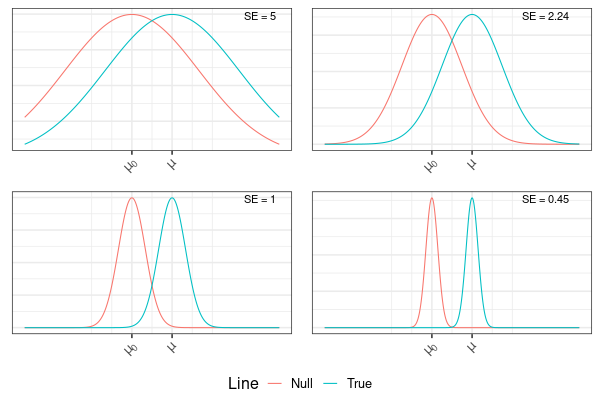
\includegraphics[scale=0.49]{null_plotter.png}
\end{center}
\end{frame}

\begin{frame}{Type II Error Rate}
The Type II error rate is typically denoted $\beta$ \vspace{4mm}

More frequently, we consider the rate at which Type II errors do not occur ($1 - \beta$), a term we refer to as \textit{power} \vspace{4mm}

A study that is unable to detect a true effect is said to be \textit{underpowered}
\end{frame}

\begin{frame}{Power}

Consider the following analogy\footnotemark: you send a child into the basement to find an object
\vspace{3mm}
\begin{itemize}
\item What is the probability that she actually finds it?
\item This will depend on three things:
	\begin{itemize}
	\item How long does she spend looking?
	\item How big is the object she is looking for?
	\item How messy is the basement?
	\end{itemize}
\end{itemize}

\footnotetext[1]{Stolen from Professor Nolte, who in turn stole this from Patrick Breheny who credits the text \textit{Intuitive Biostatistics}, which in turn credits John Hartung for this example}

\end{frame}

\begin{frame}{Power}
If the child spends a long time looking for a large object in a clean, organized basement, she will most likely find what she's looking for \vspace{4mm}

If a child spend a short amount of time looking for a small object in a messy, chaotic basement, it's probably that she won't find it \vspace{4mm}

Each of these has a statistical analog:
\begin{itemize}
\item How long she spends looking? = How big is the sample size?
\item How big is the object? = How large is the effect size?
\item How messy is the basement? = How noisy/variable is the data?
\end{itemize}
\end{frame}

\begin{frame}{Drawing Conclusions}

As we never truly know whether $H_0$ is correct or not, we must simultaneously be prepared to combat both types of error

\begin{center}
        \begin{tabular}{|l|c|c|}
        \hline
        & \multicolumn{2}{c|}{True State of Nature} \\ 
        \cline{2-3} 
        Test Result  & $H_0$ True  & $H_0$ False \\ 
        \hline
        Fail to reject $H_0$ & \begin{tabular}[c]{@{}c@{}}Correct\\ ($1 - \alpha$)\end{tabular} & 						\begin{tabular}[c]{@{}c@{}}Type II Error \\ ($\beta$)\end{tabular} \\ \hline
        Reject $H_0$         & \begin{tabular}[c]{@{}c@{}}Type I Error \\ ($\alpha$)\end{tabular} & 		\begin{tabular}[c]{@{}c@{}}Correct\\ $(1 - \beta)$\end{tabular}             \\ \hline
        \end{tabular}
\end{center}

    \begin{itemize}
        \item Type I error = $P(\text{Reject } H_0|H_0 \text{ true})$ = false alarm
        \item Type II error = $P(\text{Fail to reject } H_0|H_A \text{ true})$ = missed opportunity
	\end{itemize}

\end{frame}

\begin{frame}{Issues with Decision Making -- Significance Level}
Although the $\alpha = 0.05$ is customary for Type I error rate and a cut-off for ``statistical significance", this is no substitute for correctly evaluating context \vspace{5mm}

For example, a highly publicized study in 2009 involving a vaccine protecting against HIV found that, analyzed one way, the data suggested a $p$-value of 0.08. Computed a different way, it resulted in a $p$-value of 0.04 \vspace{5mm}

Debate and controversy ensued, primarily because the consequence of using a particular method was the difference between a result being on other side of the $p < \alpha$ threshold \vspace{5mm}

But is there really that much a difference between $p = 0.04$ and $p = 0.08$?

\begin{itemize}
    \item What about .049 and .051?
\end{itemize}
\end{frame}

\begin{frame}{Issues with Decision Making -- Significance Level}

There is an unholy obsession with using a Type I error rate of $\alpha = 0.05$ in many disciplines
\begin{itemize}
    \item the 0.05 value is arbitrary -- why 1 in 20?
\end{itemize} \vspace{4mm}

Back in the 1920s, Ronald A. Fisher (who had a big hand in making many of the methods we are covering in this class) proposed that p-values between 0.01 and 0.05 (or lower) were reasonable and he made many tables that used these cutoffs in his HUGELY famous book \textit{Statistical Methods for Research Workers}
\begin{itemize}
    \item so many scientists and statisticians followed his results that the 0.05 became incredibly common place
    \item but Fisher did not intend for everyone to use any one specific cutoff!
\end{itemize}
\end{frame}

\begin{frame}{Issues with Decision Making -- Significance Level}
Fisher intended for the signifance level $\alpha$ to be adjusted to the seriousness of getting a wrong conclusion
    \begin{itemize}
        \item does a new medication work better than another
        \begin{itemize}
            \item may want $\alpha = .01$
        \end{itemize}
        \item is the percent of red cars that drive through campus more than 10\%
        \begin{itemize}
            \item might be ok with $\alpha=.05$ or even .10
        \end{itemize}
    \end{itemize}    
\end{frame}

\begin{frame}{File Drawer Effect}
Publishing only results that show a significant finding disturbs the balance of findings in favor of positive results.\footnotemark
\vspace{4mm}

\textbf{File Drawer Effect} is when research doesn't get published because the results are not deemed significant (usually p-values $> 0.05$) \vspace{6mm}

When research is only 'publishable' if p-values are below the $\alpha$ = .05 level, it leads to lots of scientific discovery going unreported
\begin{itemize}
    \item even when we haven't found the effect we wanted to (i.e. there isn't a difference) we may have still learned something valuable!
\end{itemize}

\footnotetext[2]{Song, F.; Parekh, S.; Hooper, L.; Loke, Y. K.; Ryder, J.; Sutton, A. J.; Hing, C.; Kwok, C. S.; Pang, C.; Harvey, I. (2010). "Dissemination and publication of research findings: An updated review of related biases"}
\end{frame}

\begin{frame}{P-hacking}
\textbf{P-Hacking:} "various techniques that researchers can use to increase the chances of finding statistically significant results in their study, even if the results are not actually meaningful. This is a form of data manipulation that can lead to the publication of false positive results."\footnotemark
\begin{itemize}
    \item increasing sample size
    \begin{itemize}
        \item can detect even minute differences with very large sample sizes
        \item these small differences may not \textit{really} matter
    \end{itemize}
    \item throwing out outliers in the data set
    \item "cherry picking" - doing a whole bunch of tests and choosing the one with the smallest p-value
    \item post-data hypothesis construction
\end{itemize}
\footnotetext[3]{https://www.physiotutors.com/wiki/p-hacking/}
\end{frame}

\begin{frame}{P-hacking}
\begin{center}
"It’s critical to note that P-hacking can happen accidentally and can stem from a researcher’s lack of statistical knowledge or the pressure to publish promising results. Yet, it may also be a choice made consciously with a goal in mind. Researchers should pre-register their study design and analytic plan, report all the findings, and apply the proper statistical techniques to account for multiple comparisons in order to prevent p- hacking." \footnotemark
\end{center}

\footnotetext[4]{https://www.physiotutors.com/wiki/p-hacking/}
\end{frame}

\begin{frame}{Multiple Comparisons}
Consider conducting 8 hypothesis tests, each with a Type I error rate 5\% \vspace{4mm}


For any given test, the probability of \textit{not} making an error is
\begin{align*}
P(\text{No type I error}) = 0.95
\end{align*} \vspace{2mm}

What is the probability that I make at least one Type I error?

\vspace{-4mm}
\begin{align*}
P(\text{At least one Type I error}) &= 1 - P(\text{Probability of no Type I errors}) \\
&= 1 - (1 - 0.05)^8 = 1 - (.95)^8\\
&= 33.6\%
\end{align*} \vspace{2mm}

That is, instead of making a Type I error 1 in 20 times, we are now making it 1 in 3 times
\end{frame}

\begin{frame}{Issues in Decision Making}
The issues mentioned over the last few slide indicate that we should be a bit skeptical of the 'decision making' approach as I've described it. \vspace{4mm}

The 'strength of evidence' approach is gaining more traction, especially amongst statistics instructors.
\begin{itemize}
    \item avoids arbitrary significance thresholds
    \item encourages publication of a wider variety of results
    \item less pressure for researchers to \textit{manipulate} their data to get published
\end{itemize} \vspace{4mm}


\end{frame}

\end{document}
